\documentclass[tikz]{standalone}

\usepackage{amsmath}
\renewcommand{\vec}[1]{\boldsymbol{#1}}

\usetikzlibrary{shapes,arrows,calc,positioning,fit}

\tikzset{
  %   pinstyle/.style={pin edge={to-,thin,black}}, % you have another one below
  block/.style = {draw, rectangle,
    minimum height=1cm,
    align = center
    %   minimum width=2cm
  },
  input/.style = {coordinate,node distance=1cm},
  output/.style = {coordinate,node distance=1cm},
  arrow/.style={draw, -latex,node distance=2cm},
  pinstyle/.style = {pin edge={latex-, black,node distance=2cm}},
  sum/.style = {draw, circle, node distance=1cm},
  gain/.style = {
    regular polygon, regular polygon sides=3,
    draw, fill=white, text width=1em,
    inner sep=0mm, outer sep=0mm,
    shape border rotate=-90
  },
  dot/.style={circle,fill,draw,inner sep=0pt,minimum size=3pt}
}

\begin{document}

\begin{tikzpicture}[>=latex',every node/.append style=
      {font=\scriptsize},node distance=5mm]

    \node [input, name=input] {};
    %% \node [sum, right=of input] (speed_sum) {};
    %% \node [dot, right=8mm of speed_sum] (snodo1) {};
    %% \node [gain, above right=7mm and 5mm of snodo1] (Kp) {$K_{p}$};
    %% \node [gain, below right=7mm and 5mm of snodo1] (Ki) {$K_{i}$};

    %% \node [block,right=of Ki] (integrator) {$\frac{1}{s}$};
    %% \node [sum, xshift=7mm] at (snodo1-|integrator) (control_sum) {};
    \node [block, right=1.5cm of input] (traj_gen) {Trajectory \\ generation};
    \node [block, right=1.5cm of traj_gen] (CP) {CP \\ controller};
    \node [block, right=1.5cm of CP] (ZMP) {ZMP \\ controller};
    \node [block, right=1.5cm of ZMP] (system) {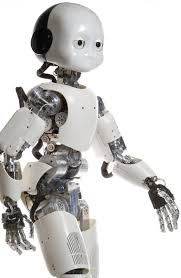
\includegraphics[scale=0.3]{icub_control_loop.jpeg}};
    \node [output, right= 1.5cm of system] (output) {};

    \node [block, below left = 0.3cm and -0.5cm of system](ZMP_eval){ZMP evaluation};
    \node [block, below left = 3cm and -1cm of ZMP](CP_eval){CP evaluation};
    
    \begin{scope}[auto]
      \draw [->] (input) -- node {Footstep} (traj_gen);
      \draw [->] (traj_gen) -- node {$\vec{\xi}_{ref}$} (CP);
      \draw [->] (CP) -- node {$\vec{p}_{ref}$} (ZMP);
      \draw [->] (ZMP) -- node {$\vec{u}_p$}(system);
      \draw [->] (system) -- node [name=robot_state] {$\vec{x}$, $\dot{\vec{x}}$, $\ddot{\vec{x}}$}
      (output);
    \end{scope}

    %DEFINIZIONE COLLEGAMENTI FEEDBACK
    \draw [->] (robot_state)  |- node [pos=0.99,right] {} (ZMP_eval);
    \draw [->] (ZMP_eval)  -| node [pos=0.7,right] {$\vec{p}$} (ZMP);

    \draw [->] (robot_state)  |- node [pos=0.99,right] {} (CP_eval);
    \draw [->] (CP_eval)  -| node [pos=0.7,right] {$\vec{\xi}$} (CP);

    %\node [dot] at (motor_speed.south) {};

 %   \draw [->] (robot_state) -- ++(0,-2)  node[left,draw] (KiKd) {Ki.Kd};
    %\draw [->] (KiKd) -- ++(0,1) -- node[above,pos=0.5] {$-$}(control_sum);

    \node [draw,dashed,fit=(ZMP)(system)(ZMP_eval)] (zmp_group) {};
    %\node [above right] at (sc.south west) {Speed controller};
  \end{tikzpicture}
\end{document}
